\documentclass[border=6pt]{standalone}
\usepackage{tikz}
\usetikzlibrary{arrows.meta,calc,decorations.pathreplacing,positioning}
\begin{document}

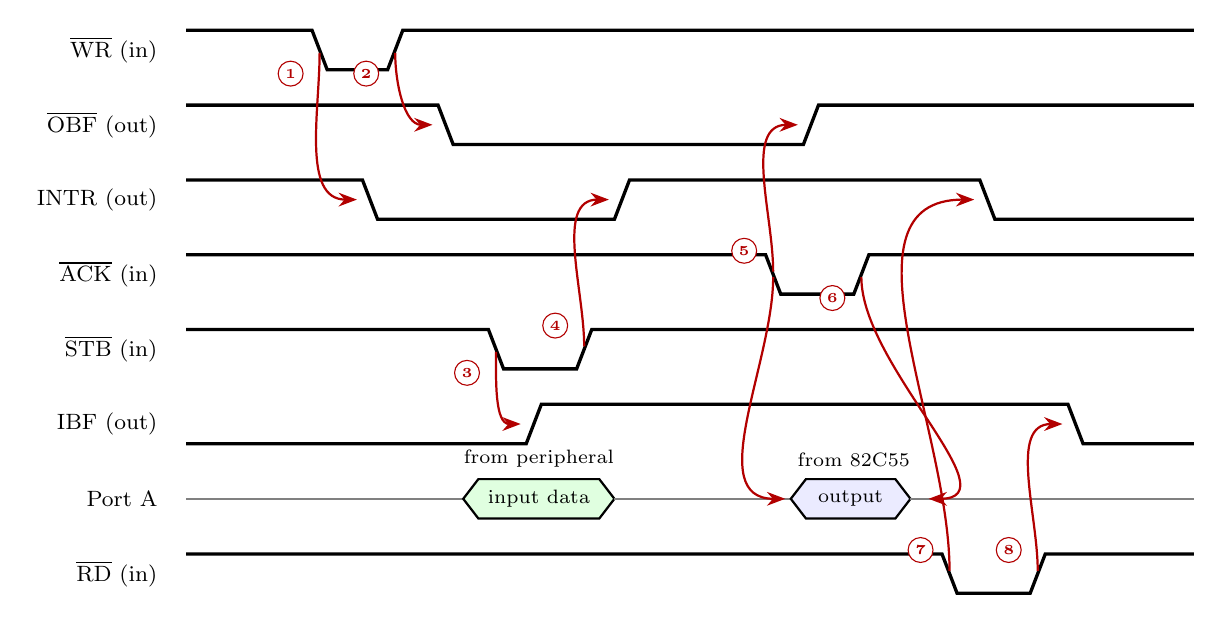
\begin{tikzpicture}[>=Stealth,font=\small,x=1.6cm,y=1cm]
% row 0 y=0
\node[anchor=east,font=\footnotesize,align=right] at (-0.15,0.25) {$\overline{\mathrm{WR}}$ (in)};
\draw[very thick] (0,0.5) -- (1,0.5) -- (1.12,0) -- (1.6,0) -- (1.72,0.5) -- (8,0.5);
% row 1 y=-0.95
\node[anchor=east,font=\footnotesize,align=right] at (-0.15,-0.7) {$\overline{\mathrm{OBF}}$ (out)};
\draw[very thick] (0,-0.45) -- (2,-0.45) -- (2.12,-0.95) -- (4.9,-0.95) -- (5.02,-0.45) -- (8,-0.45);
% row 2 y=-1.9
\node[anchor=east,font=\footnotesize,align=right] at (-0.15,-1.65) {INTR (out)};
\draw[very thick] (0,-1.4) -- (1.4,-1.4) -- (1.52,-1.9) -- (3.4,-1.9) -- (3.52,-1.4) -- (6.3,-1.4) -- (6.42,-1.9) -- (8,-1.9);
% row 3 y=-2.85
\node[anchor=east,font=\footnotesize,align=right] at (-0.15,-2.6) {$\overline{\mathrm{ACK}}$ (in)};
\draw[very thick] (0,-2.35) -- (4.6,-2.35) -- (4.72,-2.85) -- (5.3,-2.85) -- (5.42,-2.35) -- (8,-2.35);
% row 4 y=-3.8
\node[anchor=east,font=\footnotesize,align=right] at (-0.15,-3.55) {$\overline{\mathrm{STB}}$ (in)};
\draw[very thick] (0,-3.3) -- (2.4,-3.3) -- (2.52,-3.8) -- (3.1,-3.8) -- (3.22,-3.3) -- (8,-3.3);
% row 5 y=-4.75
\node[anchor=east,font=\footnotesize,align=right] at (-0.15,-4.5) {IBF (out)};
\draw[very thick] (0,-4.75) -- (2.7,-4.75) -- (2.82,-4.25) -- (7,-4.25) -- (7.12,-4.75) -- (8,-4.75);
% row 6 y=-5.7
\node[anchor=east,font=\footnotesize,align=right] at (-0.15,-5.45) {Port A};
\draw[thick,gray] (0,-5.45) -- (2.2,-5.45);
\draw[thick,fill=green!12] (2.2,-5.45) -- (2.32,-5.2) -- (3.28,-5.2) -- (3.4,-5.45) -- (3.28,-5.7) -- (2.32,-5.7) -- cycle;
\node[font=\scriptsize] at (2.8,-5.45) {input data};
\draw[thick,gray] (3.4,-5.45) -- (4.8,-5.45);
\draw[thick,fill=blue!8] (4.8,-5.45) -- (4.92,-5.2) -- (5.63,-5.2) -- (5.75,-5.45) -- (5.63,-5.7) -- (4.92,-5.7) -- cycle;
\node[font=\scriptsize] at (5.275,-5.45) {output};
\draw[thick,gray] (5.75,-5.45) -- (8,-5.45);
% row 7 y=-6.65
\node[anchor=east,font=\footnotesize,align=right] at (-0.15,-6.4) {$\overline{\mathrm{RD}}$ (in)};
\draw[very thick] (0,-6.15) -- (6,-6.15) -- (6.12,-6.65) -- (6.7,-6.65) -- (6.82,-6.15) -- (8,-6.15);
\tikzset{cz/.style={->,thick,red!70!black,shorten <=1pt,shorten >=2pt},num/.style={circle,draw=red!70!black,fill=white,font=\tiny\bfseries,text=red!70!black,inner sep=0.5pt,minimum size=9pt}}
\draw[cz] (1.06,0.25) to[out=-90,in=180] (1.4,-1.65);
\node[num] at (0.83,-0.05) {1};
\draw[cz] (1.66,0.25) to[out=-90,in=180] (2,-0.7);
\node[num] at (1.43,-0.05) {2};
\draw[cz] (2.46,-3.55) to[out=-90,in=180] (2.7,-4.5);
\node[num] at (2.23,-3.85) {3};
\draw[cz] (3.16,-3.55) to[out=90,in=180] (3.4,-1.65);
\node[num] at (2.93,-3.25) {4};
\draw[cz] (4.66,-2.6) to[out=90,in=180] (4.9,-0.7);
\node[num] at (4.43,-2.3) {5};
\draw[cz] (4.66,-2.6) to[out=-90,in=180] (4.8,-5.45);
\draw[cz] (5.36,-2.6) to[out=-90,in=0] (5.85,-5.45);
\node[num] at (5.13,-2.9) {6};
\draw[cz] (6.06,-6.4) to[out=90,in=180] (6.3,-1.65);
\node[num] at (5.83,-6.1) {7};
\draw[cz] (6.76,-6.4) to[out=90,in=180] (7,-4.5);
\node[num] at (6.53,-6.1) {8};
\node[font=\scriptsize,anchor=south] at (2.8,-5.17) {from peripheral};
\node[font=\scriptsize,anchor=south] at (5.3,-5.17) {from 82C55};
\end{tikzpicture}
\end{document}
